\documentclass[11pt,letterpaper]{article}
\usepackage[lmargin=1in,rmargin=1in,bmargin=1in,tmargin=1in]{geometry}
\usepackage{../style}

\setlength{\parindent}{0ex}

% -------------------
% Content
% -------------------
\begin{document}

\pagenumbering{gobble}

% Recitation: Linear Functions Review
\phantom{} \hfill {\bfseries \Large Recitation: Linear Functions Review} \hfill \phantom{} \par\vspace{0.5cm}

% Problem 1
\noindent {\bfseries Problem 1.} A small tanker truck is depositing its gas at a storage facility. The tanker is carrying 11,600~gallons of gas and is emptying its tank at a rate of 528.3~gal/min. Let $G(t)$ denote the volume of gas, in thousands, left in the tanker $t$ minutes from now. 
	\begin{enumerate}[(a)]
	\item Explain why $G(t)$ is linear. 
	\item Find $G(t)$ and sketch it in the plot below. 
	\item Interpret the slope of $G(t)$.
	\item Interpret the $y$-intercept for $G(t)$.
	\item Find and interpret (if possible) the $x$-intercept for $G(t)$. 
	\end{enumerate}
	
	\vfill

	\hfill \fbox{
	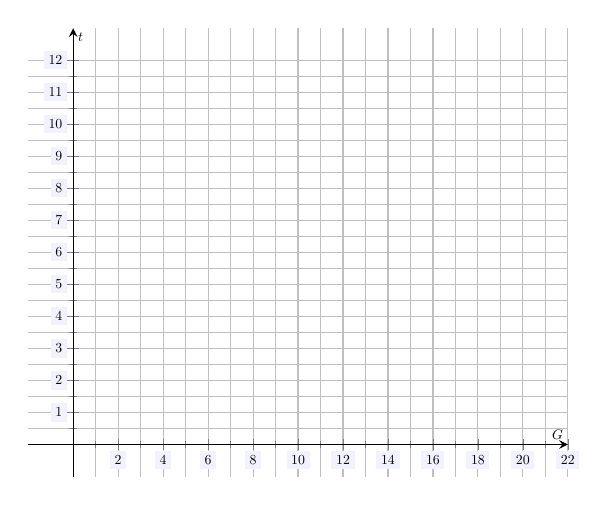
\begin{tikzpicture}[scale=1,every node/.style={scale=0.5}]
	\begin{axis}[
	grid=both,
	axis lines=middle,
	ticklabel style={fill=blue!5!white},
	xmin= -2, xmax=22,
	ymin= -1, ymax=13,
	xtick={0,2,...,22},
	ytick={0,1,2,...,12},
	minor x tick num = 1,
	minor y tick num = 1,
	xlabel=\(G\),ylabel=\(t\),
	]
	\end{axis}
	\end{tikzpicture}
	}
	


\newpage



% Problem 2
\noindent {\bfseries Problem 2.} Find the equation of the line with $x$-intercept 5 and $y$-intercept $-6$. \par\vspace{2.5in}



% Problem 3
\noindent {\bfseries Problem 3.} Consider the linear function $\ell(x)= \tfrac{3x - 5}{4}$. 
	\begin{enumerate}[(a)]
	\item Find the slope and $y$-intercept for $\ell(x)$.
	\item Find the $x$-intercept(s) of $\ell(x)$.
	\item Is $(-1, 2)$ on the graph of $\ell(x)$?
	\item Compute $\ell(1)$.
	\item Determine the domain and range for $\ell(x)$.
	\end{enumerate}

\vfill

\end{document}